%<dscrpt>Disque elliptique comme union de cercles.</dscrpt>
\noindent
Un plan $\mathcal P$ est muni d'un repère orthonormé. L'affixe complexe d'un point est relative à ce repère.\newline
L'objet de ce problème est de préciser, pour des nombres complexes $a$, $b$, $c$ fixés ($a\neq b$), l'ensemble (noté $\mathcal D$) des points du plan dont l'affixe complexe appartient à
\begin{displaymath}
 \left\lbrace a|z_1|^2 + b|z_2|^2 + cz_1\overline{z_2}, (z_1,z_2)\in \C^2 \text{ tq } |z_1|^2 + |z_2|^2 = 1 \right\rbrace 
\end{displaymath}

\subsection*{Partie I. Ellipses.}
Dans cette partie, $a$ et $b$ sont des réels tels que $0 < b < a$.
\begin{enumerate}
  \item Soit $(x,y,z) \in \R^3$. Pour $c$ et $d$ réels, on considère l'expression  
\[
  \frac{1}{b^2}\left( (x-cz)^2 + y^2\right) -\left( \frac{1}{b^2}-\frac{1}{a^2}\right) (x - dz)^2. 
\]
\begin{enumerate}
  \item Préciser le coefficient de $xz$ et celui de $z^2$ dans le développement de l'expression au dessus.
  \item Déterminer $c$ et $d$ réels positifs tels que, pour tous $x$, $y$ réels,
\begin{multline*}
\frac{1}{a^2}\,x^2 + \frac{1}{b^2}\,y^2 - 1 
= \frac{1}{b^2}\left( (x-c)^2 + y^2\right) -\left( \frac{1}{b^2}-\frac{1}{a^2}\right) (x - d)^2\\
= \frac{1}{b^2}\left( (x+c)^2 + y^2\right) -\left( \frac{1}{b^2}-\frac{1}{a^2}\right) (x + d)^2.
\end{multline*}
  \item  Montrer que $0 < c < a < d$. On note $e = \frac{c}{a}$. Vérifier que $a = ed$.
\end{enumerate}
\item Montrer que, pour tout $x$ et $y$ réels,
\[
  \frac{x^2}{a^2} + \frac{y^2}{b^2} = 1
  \Leftrightarrow 
  (x-c)^2 + y^2 = e^2(x-d)^2
  \Leftrightarrow
  (x + c)^2 + y^2 = e^2(x + d)^2.
\]
\setcounter{numquestion}{\value{enumi}}
\end{enumerate}
On introduit des points $F_+$ et $F_-$ respectivement de coordonnées $(c,0)$ et $(-c,0)$.\newline
On note $\mathcal{E}$ l'ensemble des points dont les cordonnées $(x,y)$ vérifient 
\[
  \frac{x^2}{a^2} + \frac{y^2}{b^2} = 1 .
\]
Le tableau suivant définit le vocabulaire usuel dans ce cadre
\begin{center}
\renewcommand{\arraystretch}{1.3}
\begin{tabular}{|c|c|c|p{2cm}|c|c|}\hline
ellipse       & excentricité    & foyers             & \centering directrices                                      & grand axe & petit axe\\ \hline
$\mathcal{E}$ & $e=\frac{c}{a}$ & points $F$ et $F'$ & \centering droites d'equ \newline $x = d$,\newline $x = -d$ & $2a$      & $2b$ \\ \hline
\end{tabular}
\end{center}

\begin{enumerate}
  \setcounter{enumi}{\value{numquestion}}
  \item Soit $M$ un point de coordonnées $(x,y)$.
  \begin{enumerate}
    \item Montrer que $M\in \mathcal{E}$ entraine $|x| \leq a$.
    \item Montrer les équivalences suivantes:
\[
  M\in \mathcal{E}
  \Leftrightarrow MF_+ = e(d-x) \Leftrightarrow MF_- = e(d+x) \Leftrightarrow MF_+ + MF_- = 2a.
\]
  \end{enumerate}
  \setcounter{numquestion}{\value{enumi}}
\end{enumerate}
Il est clair que pour tout réel $t$, le point de coordonnées $(a\cos t, b\sin t)$ appartient à $\mathcal{E}$. On en déduit le tracé de cette courbe (ellipse).\newline
La figure \ref{fig:disqell_1} présente des ellipses de mêmes foyers $F$ et $F'$ ( avec $c = 1$) et de demi-grand-axe $a$ entre 1.05 et 1.25
\begin{figure}[h!]
  \centering
  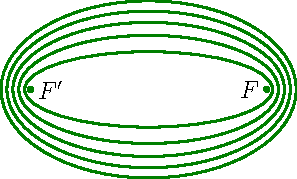
\includegraphics{Edisqell_1.pdf}
  % Edisqell_1.pdf: 114x58 px, 72dpi, 4.02x2.05 cm, bb=0 0 114 58
  \caption{Ellipses homofocales}
  \label{fig:disqell_1}
\end{figure}

\begin{enumerate}
  \setcounter{enumi}{\value{numquestion}}
  \item Soit $u$ et $v$ deux nombres complexes avec $u\neq 0$ et $S$ l'application de $\mathcal P$ dans $\mathcal P$ qui à un point $M$ d'affixe $z$ associe le point $S(M)$ d'affixe $uz+v$.\newline
 On note $\mathcal E ^\prime$ l'image de $\mathcal E$ par $S$. Préciser les points $F_+'$, $F_-'$ et le réel positif $a'$ tel que
\[
\forall m \in \mathcal{P},\;  M \in \mathcal{E}' \Leftrightarrow MF_+' + MF_-' = 2a'.
\]
\end{enumerate}

\subsection*{Partie II. Cercles.}
\begin{enumerate}
\begin{figure}[ht]
 \centering
 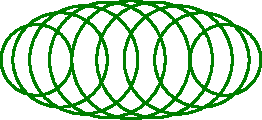
\includegraphics{Edisqell_2.pdf}
 \caption{Tracé de quelques $\mathcal C_\rho$ pour $\lambda=1$.}
 \label{fig:Edisqell_2}
\end{figure}
\item Dans cette question $\lambda > 0$, $\rho\in ]0,1[$ et $\mathcal C_\rho$ est le cercle défini par:
\begin{align*}
 \text{affixe du centre : } -1+2\rho & & \text{rayon : } \lambda\sqrt{\rho - \rho^2}.
\end{align*}
 \begin{enumerate}
 \item Former un équation de $\mathcal C_\rho$.
 \item Montrer que l'ensemble (noté $\mathcal E_\lambda$) des points du plan par lesquels \emph{passe exactement} un cercle $\mathcal C_\rho$ est une conique dont on donnera une équation réduite. Préciser le centre, l'axe focal et les foyers.
 \item Quel est l'ensemble (noté $\Delta _\lambda)$ des points par lesquels passe au moins un cercle $\mathcal C_\rho$ ?
 \end{enumerate}

\item Soit $S$ la fonction du plan dans lui même qui à un point d'affixe $z$ associe le point d'affixe 
\begin{displaymath}
 \dfrac{2}{a-b}z-\dfrac{a+b}{a-b}
\end{displaymath}

\begin{enumerate}
 \item Montrer que $S$ est bijective. Préciser la bijection réciproque notée $S^\prime$.
 \item Quelle est l'image par $S$ d'un cercle de centre $C$ et de rayon $r$?
 \item Soit $r\in]0,1[$, montrer que l'image par $S$ d'un cercle vérifiant
  \begin{align*}
 \text{affixe du centre : } ar^2+b(1-r^2) & &  \text{rayon : } |c|r\sqrt{1-r^2}
  \end{align*}
est un cercle $\mathcal C_\rho$ pour des $\rho$ et $\lambda$ à préciser en fonction de $a$, $b$, $c$.
\end{enumerate}

 \item Soit $r\in]0,1[$ fixé, montrer que l'ensemble des points d'affixe
\begin{align*}
 a|z_1|^2 + b|z_2|^2 +cz_1\overline{z_2} & & \text{ avec } & & |z_1|^2+|z_2|^2 = 1 & &  \text{ et }  & & |z_1| =r 
\end{align*}
est un cercle.  Préciser son centre et son rayon.

\item Montrer que $\mathcal D$ est l'image par $S^\prime$ d'un ensemble $\mathcal E_\lambda$ pour un $\lambda$ à exprimer en fonction de $a$, $b$, $c$. Pour ce $\lambda$, quels sont les foyers de $S^\prime(\mathcal E_\lambda)$ ?
\end{enumerate}
